\documentclass[12pt]{article}

\usepackage[margin=.8in,letterpaper]{geometry}
\usepackage{enumitem}
\usepackage{graphicx}
\usepackage{tikz}%,graphicx,wrapfig}
\usepackage{mathpazo}
\usepackage[scaled]{helvet}
\usepackage{siunitx}
\usepackage{multicol}

\usetikzlibrary{decorations.pathmorphing,patterns}

\sisetup{number-math-rm=\mathnormal}

\renewcommand{\familydefault}{\sfdefault}

\newcommand{\pic}[2]{\includegraphics[width=#1\textwidth]{#2}}
\newcommand{\magdir}[2]{$#1\;[\mathrm{#2}]$}
\newcommand{\mb}[1]{\mathbf{#1}}

\begin{document}

\begin{center}
  Student \#: \underline{\hspace{1in}}\hspace{1.9in}
  Student Name: \underline{\hspace{2in}}\\
  \vspace{0.3in}
  {\LARGE
    AP Physics \hspace{0.68in} Class 7: Simple Harmonic Motion
  }
\end{center}

%\noindent On all of the questions in this book, you may neglect air resistance
%and use $g =\SI{10}{m/s^2}$ unless otherwise noted.

%\begin{multicols}{2}
\begin{enumerate}[leftmargin=50pt,label=\underline{\hspace{0.4in}} \arabic*.]

\item A simple pendulum has a mass $m$, length $L$, and period $T$. If the
  pendulum mass is replaced by a mass of $2m$, the period will be
  \begin{enumerate}[noitemsep,topsep=0pt]
  \item doubled
  \item halved
  \item quartered
  \item quadrupled
  \item unchanged
  \end{enumerate}

\item A mass oscillates on the end of a spring that obeys Hooke's law. Which of
  the following statements is true?
  \begin{enumerate}[noitemsep,topsep=0pt,leftmargin=18pt]
  \item The amplitude of oscillation is equal to the potential energy of the
    spring.
  \item The kinetic energy of the oscillating mass is constant.
  \item Maximum potential energy occurs when the mass reaches the
    equilibrium position.
  \item The potential energy of the spring at the amplitude is equal to the
    kinetic energy at the equilibrium position.
  \item The kinetic energy of the spring at the amplitude is equal to the
    potential energy at the equilibrium position.
  \end{enumerate}

\item A superball is dropped from a height of \SI{5.0}{meters} above a floor.
  The ball bounces off the floor in a perfectly elastic collision so that it
  rises to the same height with each bounce. The motion of the ball can be
  described as
  \begin{enumerate}[noitemsep,topsep=0pt]
  \item harmonic motion with a period of $2$ \si{s}
  \item harmonic motion with a period of $1$ \si{s}
  \item harmonic motion with a period of $1/2$ \si{s}
  \item motion with a constant velocity
  \item motion with a constant momentum
  \end{enumerate}

\item An object oscillates in simple harmonic motion along the $x$-axis
  according to the equation $x = 6 \cos(4t)$. The period of oscillation of the
  object is
  \begin{enumerate}[noitemsep,topsep=0pt]
  \item $1/4$ \si{s}
  \item\SI{4}{s}
  \item\SI{\pi/4}{s}
  \item\SI{\pi/2}{s}
  \item\SI{4\pi}{s}
  \end{enumerate}    

\item A mass $m$ oscillates on the end of a string of length $L$. The frequency
  of the pendulum is $f$. How would you increase the frequency of the
  pendulum to $2f$?
  \begin{enumerate}[noitemsep,topsep=0pt]
    \item Increase the length of the pendulum to $4L$
    \item Decrease the length of the pendulum to $1/4L$
    \item Increase the length of the pendulum to $2L$
    \item Decrease the length of the pendulum to $1/2L$
    \item Decrease the mass of the pendulum to $1/2m$
  \end{enumerate}

  \vspace{-0.1in}\begin{center}
    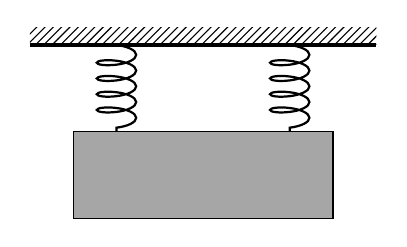
\begin{tikzpicture}[scale=1.1]
      \fill [pattern=north east lines] (-2,4) rectangle (2,4.2);
      \draw[ultra thick] (-2,4)--(2,4);
      \draw[thick,
        decoration={aspect=0.3,segment length=2mm, amplitude=2.5mm, coil},
        decorate] (-1,4)--(-1,3);
      \draw[thick,
        decoration={aspect=0.3,segment length=2mm, amplitude=2.5mm, coil},
        decorate] (1,4)--(1,3);
      \draw[fill=gray!70](-1.5,3) rectangle(1.5,2);
    \end{tikzpicture}
  \end{center}

\item\vspace{-.2in} A mass hangs from two parallel springs, each with the same spring
  constant $k$. Compared to the period $T$ of the same mass oscillating on
  one of the springs, the period of oscillation of the mass with both
  springs connected to it is
  \begin{enumerate}[noitemsep,topsep=0pt]
  \item $1/4T$
  \item $1/2T$
  \item $T$ (unchanged)
  \item $2T$
  \item $4T$
  \end{enumerate}

\item Which of the following is generally true for an object in simple
  harmonic motion on a spring of constant k?
  \begin{enumerate}[noitemsep,topsep=0pt]
  \item The greater the spring constant $k$, the greater the amplitude of the
    motion.
  \item The greater the spring constant $k$, the greater the period of the
    motion.
  \item The greater the spring constant $k$, the greater the frequency of the
    motion.
  \item The lower the spring constant $k$, the greater the frequency of the
    motion.
  \item The lower the spring constant $k$, the greater the kinetic energy of
    the motion.
  \end{enumerate}
\end{enumerate}

\noindent Questions 8-10: A harmonic oscillator follows the equation
$\displaystyle\frac{d^2x}{dt^2}=-4x$. The spring constant $k$ is \SI{4}{N/m}.

\begin{enumerate}[leftmargin=50pt,label=\underline{\hspace{0.4in}} \arabic*.]
  \setcounter{enumi}{7}
\item The angular frequency ω of the harmonic motion is
  \begin{enumerate}[noitemsep,topsep=0pt]
  \item zero
  \item\SI{2}{rad/s}
  \item\SI{4}{rad/s}
  \item\SI{8}{rad/s}
  \item\SI{16}{rad/s}
  \end{enumerate}

\item The mass $m$ oscillating on the spring is
  \begin{enumerate}[noitemsep,topsep=0pt]
  \item\SI{1}{\kg}
  \item\SI{2}{\kg}
  \item\SI{4}{\kg}
  \item\SI{8}{\kg}
  \item\SI{16}{\kg}
  \end{enumerate}
  
\item The period $T$ of oscillation is
  \begin{enumerate}[noitemsep,topsep=0pt]
  \item zero
  \item $\pi/4$\si{s}
  \item $\pi/2$\si{s}
  \item $\pi$  \si{s}
  \item $2\pi$ \si{s}
  \end{enumerate}

\item A pendulum of length $L$ has a period of \SI{2}{\s} on Earth. A planetary
  explorer takes the same pendulum of length $L$ to another planet where
  its period is \SI{1}{\s}. The gravitational acceleration on the surface of
  this planet is most nearly
  \begin{enumerate}[noitemsep,topsep=0pt]
  \item $8 g$
  \item $4 g$
  \item $2 g$
  \item $1⁄2 g$
  \item $1⁄4 g$
  \end{enumerate}

  \vspace{-.45in}\begin{center}
    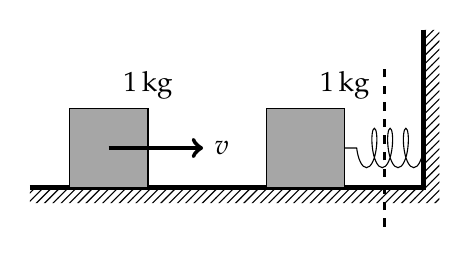
\begin{tikzpicture}
      \fill [pattern=north east lines] (-5,0)--(0,0)--(0,2)--(0.2,2)--(0.2,-0.2)
      --(-5,-0.2)--cycle;
      \draw[ultra thick] (-5,0)--(0,0)--(0,2);
      \draw[decoration={aspect=0.3,segment length=2mm, amplitude=2.5mm, coil},
        decorate] (0,0.5)--(-1,0.5);
      \draw[fill=gray!70](-2,0) rectangle(-1,1) node[above]{\SI{1}{\kg}};
      \draw[fill=gray!70](-4.5,0) rectangle(-3.5,1) node[above]{\SI{1}{\kg}};
      \draw[ultra thick,->](-4,0.5)--(-2.8,0.5) node[pos=1,right]{$v$};
      \draw[very thick,dashed](-0.5,-0.5)--(-0.5,1.5);
    \end{tikzpicture}
  \end{center}
  
\item\vspace{-0.2in} A block of mass \SI{1.0}{\kg} is sliding on a frictionless
  horizontal
  surface with a speed of \SI{4.0}{m/s} when it collides inelastically with
  another \SI{1.0}{kg} block attached to a spring. The spring compresses a
  distance of \SI{0.5}{m} after the collision. The force constant $k$ of the
  spring is
  \begin{enumerate}[noitemsep,topsep=0pt]
  \item\SI{2}{N/m}
  \item\SI{4}{N/m}
  \item\SI{8}{N/m}
  \item\SI{16}{N/m}
  \item\SI{32}{N/m}
  \end{enumerate}

  \begin{center}
    \pic{0.45}{projectile.png}
  \end{center}
  
\item A block of mass \SI{0.5}{kg} rests up against a compressed spring of force
  constant \SI{5}{N/m}. The spring is released, and the block travels a distance
  of \SI{1.0}{m} when the block leaves the spring at the edge of the horizontal
  frictionless table, and is projected to the floor. The table is \SI{1.5}{m}
  high. The horizontal distance from the table the block lands on the floor is
  \begin{enumerate}[noitemsep,topsep=0pt]
  \item\SI{1.2}{\metre}
  \item\SI{1.7}{\metre}
  \item\SI{2.1}{\metre}
  \item\SI{2.8}{\metre}
  \item\SI{3.4}{\metre}
  \end{enumerate}
\end{enumerate}

\newpage
\noindent The following questions are ``review'' questions for kinematics.

\begin{enumerate}[leftmargin=50pt,label=\underline{\hspace{0.4in}} \arabic*.]
  \setcounter{enumi}{13}

\item  A golf ball is hit from level ground and has a horizontal range of
  \SI{100}{m}. The ball leaves the golf club at an angle of \ang{60} to the
  level ground. At what other angle(s) can the ball be struck at the same
  initial velocity and still have a range of \SI{100}{m}?
  \begin{enumerate}[noitemsep,topsep=0pt]
  \item\ang{30}
  \item\ang{20} and \ang{80}
  \item\ang{10} and \ang{120}
  \item\ang{45} and \ang{135}
  \item There is no other angle other than \ang{60} in which the ball will have
    a range of \SI{100}{m}.
  \end{enumerate}

  \vspace{-.23in}\begin{center}
    \pic{0.3}{golf.png}
  \end{center}

\item\vspace{-.2in}A particle moves on a horizontal surface with a constant acceleration of
  \SI{6}{m/s^2} in the $x$-direction and \SI{4}{m/s^2} in the $y$-direction. The
  initial velocity of the particle is \SI{3}{m/s} in the $x$-direction.
  The speed of the particle after \SI{4}{s} is
  \begin{enumerate}[noitemsep,topsep=0pt]
  \item\SI{16}{m/s}
  \item\SI{27}{m/s}
  \item\SI{31}{m/s}
  \item\SI{44}{m/s}
  \item\SI{985}{m/s}
  \end{enumerate}

\item The displacement of the particle (from the previous question) from its
  initial position is
  \begin{enumerate}[noitemsep,topsep=0pt]
  \item\SI{16}{\metre}
  \item\SI{32}{\metre}
  \item\SI{60}{\metre}
  \item\SI{68}{\metre}
  \item\SI{92}{\metre}
  \end{enumerate}

  \vspace{-0.5in}\begin{center}
    \pic{0.3}{bounce.png}
  \end{center}
  
\item\vspace{-.2in} A rubber ball is dropped from rest onto a plane angled at \ang{30} to the
  horizontal floor and bounces off the plane with a horizontal speed $v_o$.
  The ball lands on the plane a distance $D$ along the plane, as shown above.
  In terms of $v_o$, $D$, and $g$, the speed of the ball just before striking
  the plane is
  \begin{enumerate}[noitemsep,topsep=0pt]
  \item $v_o$
  \item $\displaystyle\left(v_o^2+2D\sin\theta g\right)^\frac{1}{2}$
  \item $\displaystyle\left(v_o+\frac{D\sin\theta}{g}\right)^\frac{1}{2}$
  \item $\displaystyle\left(v_o^2+\frac{D\sin\theta}{g}\right)^\frac{1}{2}$
  \item $\displaystyle\left(2D\sin\theta g\right)^\frac{1}{2}$
  \end{enumerate}

  \vspace{-.2in}\begin{center}
    \pic{.55}{projectile2.png}
  \end{center}

\item\vspace{-.2in} A projectile is launched from a platform \SI{20}{m} high above level
  ground. The projectile is launched with a velocity of \SI{40}{m/s} at an
  angle of \ang{60} above the horizontal. The projectile follows a parabolic
  path and reaches its original height at a horizontal distance of \SI{80}{m},
  but moves past the height of the cliff to strike the ground below. The total
  time from the launch until it strikes the ground is
  \begin{enumerate}[noitemsep,topsep=0pt]
  \item\SI{2}{\second}
  \item\SI{4}{\second}
  \item\SI{6}{\second}
  \item\SI{9}{\second}
  \item\SI{10}{\second}
  \end{enumerate}

 \vspace{-.45in}\begin{center}
   \pic{.45}{cup.png}
 \end{center}

\item\vspace{-.2in}A small ball is launched with a speed of \SI{8}{m/s} at an angle of
  \ang{30} from the horizontal. A cup is hung so that it is in position to
  catch the ball when it reaches its maximum height. How far above the floor
  should the cup be hung to catch the ball?
  \begin{enumerate}[noitemsep,topsep=0pt]
  \item\SI{2.4}{\metre}
  \item\SI{1.6}{\metre}
  \item\SI{1.0}{\metre}
  \item\SI{0.8}{\metre}
  \item\SI{0.4}{\metre}
  \end{enumerate}

\item A small airplane can fly at \SI{200}{km/h} with no wind. The pilot of the
  plane would like to fly to a destination \SI{100}{\km} due north of his
  present position, but there is a crosswind of \SI{50}{km/h} east. How much
  time is required for the plane to fly north to its destination?
  \begin{enumerate}[noitemsep,topsep=0pt]
  \item less than \SI{1/2}{h}
  \item \SI{1/2}{h}
  \item more than \SI{1/2}{h}
  \item \SI{1}{h}
  \item more than \SI{1}{h}
  \end{enumerate}

\end{enumerate}

\newpage
\noindent\textbf{Free-Response Questions:}

\begin{enumerate}[leftmargin=15pt]

\item A mass $m$ oscillates on an ideal spring of spring constant $k$ on a
  frictionless horizontal surface. The mass is pulled aside to a distance $A$
  from its equilibrium position, and released.
  \begin{center}
    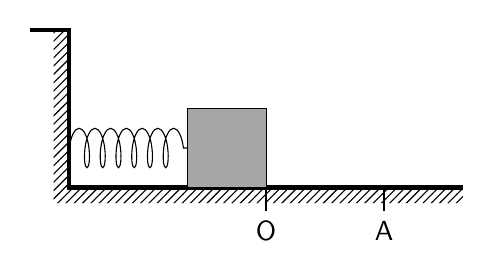
\begin{tikzpicture}
      \fill [pattern=north east lines] (5,0)--(0,0)--(0,2)--(-0.2,2)
      --(-0.2,-0.2)--(5,-0.2)--cycle;
      \draw[ultra thick] (5,0)--(0,0)--(0,2)--(-0.5,2);
      \draw[decoration={aspect=0.3,segment length=2mm, amplitude=2.5mm, coil},
        decorate] (0,0.5)--(1.5,0.5);
      \draw[fill=gray!70](1.5,0) rectangle(2.5,1);
      \draw[thick](2.5,0)--(2.5,-0.3) node[pos=1,below]{O};
      \draw[thick](4,0)--(4,-0.3) node[pos=1,below]{A};
    \end{tikzpicture}
  \end{center} 
  \begin{enumerate}[noitemsep]  
  \item In terms of the given quantities, at what distance from the equilibrium
    position is the potential energy of the mass equal to its kinetic energy?
  \item In terms of the given quantities, what is the acceleration of the mass
    when it is at the amplitude $A$?
  \end{enumerate}
%  \vspace{3in}
  \newpage
  
\item A mass oscillates in simple harmonic motion as shown by the position $x$
  vs. time $t$ graph below.
  \begin{center}
    \pic{.45}{oscillate.png}
  \end{center}
  \begin{enumerate}[noitemsep]  
  \item What is the frequency of oscillation?
  \item Write the equation that represents the speed of the mass as a function
    of time.
  \end{enumerate}
  \newpage

\item The acceleration vs.\ time graph shows the motion of an elevator during a
  $20$-second time interval. The elevator starts from rest at time $t=0$. 
  \begin{center}
    \pic{.7}{a-t.png}
  \end{center}
  \begin{enumerate}[noitemsep]
  \item Determine the instantaneous velocity of the elevator at the end of
    \SI{10}{s}.
    \vspace{1.5in}
  \item Determine the displacement of the elevator after \SI{5}{s}.
    \vspace{1.5in}
  \item On the axes below, sketch the graph that represents the velocity vs.\
    time graph for the elevator for the $20$-second time interval.
    \begin{center}
      \pic{.8}{v-t.png}
    \end{center}
    \newpage
  \end{enumerate}
  
\item A particle follows a parabolic path with the equation $y=2x^2$ as shown.
  The $x$-component of the particle's velocity $v_x$ as a function of time $t$
  is $6$, that is, the horizontal displacement is $x=6t$.
  \begin{center}
    \begin{tikzpicture}[scale=1.6]
      \draw[very thick,->](0,0)--(5,0) node[pos=1,right]{$x$};
      \draw[very thick,->](0,0)--(0,4) node[pos=1,above]{$y$};
      \draw[very thick,smooth,samples=20,domain=0:4.2] plot(\x,{.2*\x*\x});
      \draw[fill=black](3,1.8) circle(0.05) node[right]{$P$};
    \end{tikzpicture}
  \end{center}
  \begin{enumerate}[noitemsep]
  \item Determine the $y$-component of the particle's velocity $v_y$ as a
    function of time.
  \item On the diagram above, sketch arrows to represent the horizontal and
    vertical components of the particle's acceleration at point $P$.
  \end{enumerate}
\end{enumerate}
\end{document}
